
% a new beamer file for prague workshop

%% 
%%	This is file 'beamer_sample.tex'
%%	according to an MPIDR's PowerPoint template (?)
%%	
%%	by Eric Naujoks
%%
%%	Problems, bugs and comments to 
%%	naujoks@demogr.mpg.de
%%

%%%%%%%%%%%%%%%%%%%%%%%%%%%%%%%%%%
%%	Praelegomena								%%
%%%%%%%%%%%%%%%%%%%%%%%%%%%%%%%%%%
%%	- Make sure that you use utf8-encoding for all your .tex-files!!! (TeXnicCenter since version 2.0)
%%	- TeXnicCenter update: MPIDR intranet > Hard- & Sortfware > Software > Script and text editors > TeXnicCenter

\documentclass[20pt]{beamer}

\usepackage[ngerman,english]{babel}
\usepackage{graphicx}
\usepackage{tikz}
\usepackage{animate} 
\usepackage[normalem]{ulem}
\geometry{paperwidth=10in, paperheight=7.5in}
\usepackage{hyperref}
\usepackage[utf8]{inputenc}
\usepackage{multirow}
\usepackage{movie15}
%\usepackage{multimedia}
\usepackage{caption}
\captionsetup[figure]{labelformat=empty}
\usepackage[mpidr]{./mpidr/beamerthemeMPIDR}
\usepackage{array}
\newcolumntype{L}[1]{>{\raggedright\let\newline\\\arraybackslash\hspace{0pt}}m{#1}}
\newcolumntype{C}[1]{>{\centering\let\newline\\\arraybackslash\hspace{0pt}}m{#1}}
\newcolumntype{R}[1]{>{\raggedleft\let\newline\\\arraybackslash\hspace{0pt}}m{#1}}


%% Declaring title and author
\title{Morbidity and Mortality}
\subtitle{Tim Riffe\\ Pil H. Chung\\ John MacInnes}
%% subtitle means author in this file...
% :/
%%	the institute's logo
\renewcommand{\mylogo}{
\includegraphics[width=5in]{logocustom}}


%%	should be the very last package to be loaded
\usepackage{hyperref}

%%%%%%%%%%%%%%%%%%%%%%%%%%%%%%%%%%
%%	Beginning of the document		%%
%%%%%%%%%%%%%%%%%%%%%%%%%%%%%%%%%%
\begin{document}
%%	titlepage - fixed frame:
%%	========================
\begin{frame}
	\titlepage
\end{frame}


% typical APC setup
\begin{frame}
\frametitle{A test title}
\begin{figure}[b]
    \centering
       % figure made in R/TetraCombos.R
    %\includegraphics{Figures/Tetra1prg.pdf}
\end{figure} 
\end{frame}
%%	====
\begin{frame}%{Table of Contents}
\frametitle{The problem}
  \begin{description}
    \item<1->{\textbf{Projections}} show population \textbf{ageing}.
    \item<2->{\textbf{Robust}} mortality data, good projections.
    \item<3->{\textbf{Less reliable}} data on health. Less comparable.
    Cross-sectional surveys, subjective responses. Excluded populations.
    \item<4->{\textbf{Age-specific}} morbidity estimates key for predicting
    consequences of population ageing--- Social and health care demands.
  \end{description}
\end{frame}	



\begin{frame}
\frametitle{Some morbidity scenarios}
* assume mortality declines gradually, or similar.
\begin{block}{Expansion}
\begin{description}
\item[1)] ASMR\footnotemark $\uparrow$ (or
const) = morbidity vol. $\uparrow$
\item[2)] ASMR $\downarrow$ but insufficient to offset mortality
                  decline = morbidity vol. $\uparrow$
\end{description}
\end{block}

\begin{block}{Compression}
\begin{description}
\item[3)]ASMR $\downarrow$ fully offsets increased surv = constant morbidity
vol.
\item[4)] Fall in ASMRs outstrips mortality decline = morbidity vol. $\downarrow$
\end{description}
\end{block}
\footnotetext{ASMR is age-specific morbidity here}
\end{frame}	

%%	section 1:
\begin{frame}%{Table of Contents}
\frametitle{Literature}

\begin{block}{poor predictor}
Current ASMR may be poor predictor of future ASMR
\end{block}

\begin{block}{Behaviours}
Impact of health behaviours: smoking, obesity, education, \ldots
\end{block}

\begin{block}{Innovation}
Tech innovation can change healthcare demand for given morbidity
\end{block}

\begin{block}{Pessimism}
General Pessimism, esp. using secenario 1 (ASMR $\uparrow$, Surv $\uparrow$)
\end{block}
\end{frame}	%\end{frame}
%
\begin{frame}
\frametitle{more problems}
\begin{block}{Age standardization}
Chronological age standardization of conditions that are related with death can
degrade data rather than purge it of structure. Serious consequences.
\end{block}
\begin{block}{Assumptions}
\textbf{Chronological} age standardization makes morbidity follow OADR
\textbf{Thanatological} age standardization makes morbidity follow REDR, or
similar.\footnotemark
\end{block}
%
\footnotetext{Remember that finding about populations growing younger and older
at the same time? Morbidity measurement needs to follow that\ldots}
\end{frame}

\begin{frame}
\frametitle{OADR and REDR 1958-2009 various countries}
\begin{figure}[b]
    \centering
      % figure made in R/APClab.R
    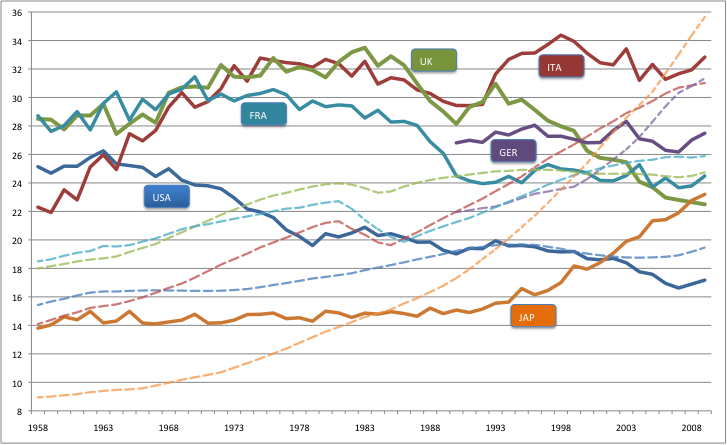
\includegraphics[scale=.9]{Figures/Johnsfig.png}
    %\caption{Lifelines in the APC diagram}
\end{figure} 
\end{frame}
\end{document}











